
\section{Introduction}
\label{sec:intro}

%high D data is growing %this is scalability challenge 
Rapid growth in high-dimensional data from automated data sources poses a scalability challenge for machine learning pipelines~\cite{plato,macrobase-cidr}.
Thus, practitioners turn to dimensionality reduction (DR) techniques to alleviate this challenge~\cite{keogh-indexing,local-dr,decade,gemini}.
%DR can help <explain>
%Dimensionality reduction (DR) techniques can alleviate this scalability challenge~\cite{keogh-indexing,local-dr,decade,gemini}.
DR methods transform an $n$-dimensional dataset to a lower $k$-dimensional representation while preserving salient dataset features.
This allows downstream analytics routines to run in time that scales with $k$, while preserving downstream task accuracy.
Thus, in exchange for a preprocessing overhead, DR techniques enable us to decrease end-to-end workload runtime.

%As downstream takss run in time that scales with k, we want k as low as possible while preserving downstream accuracy

% To attain as low a transformation dim as possible, PCA is blah blah blah
%PCA is what people want, but it is slow
To attain a target downstream task accuracy with as low a transformation dimension $k$ as possible, Principal Component Analysis (PCA) is often practioners' DR method of choice ~\cite{jolbook}. 
However, classic task-independent PCA implementations (i.e., via Singular Value Decomposition or SVD) scale poorly, with overheads that outweigh DR's downstream runtime benefit. 
In response, practitioners may use faster DR techniques that return higher $k$ for a given accuracy, but provide a lower end-to-end runtime. 
For instance, PCA is traditionally considered too computationally expensive for time series similarity search~\cite{time-series-dm}, with widely-cited work excluding it for more efficient,  less precise methods~\cite{keogh-study}. 

%Recently, the ML literature has proposed a range of stochastic methods for optimizing PCA. The high level idea is we can do PCA on samples, essentially running SGD. You can run until convergence, but this can be a waste of effort, because downstream tasks often don't need an optimal basis. For example, if I want to find nearest neighbors, can deal with approximations. So, given a dataset and downstream query, it's not clear how many iterations to run, which leads to an uncomfortable trade-off between getting the right answer unnecessarily slow and getting the wrong answer quickly.

\begin{comment}
In this work, we accelerate PCA by using this insight  regarding end-to-end workloads---that practitioners are willing to trade dimensionality for whole workload runtime.
While recent stochastic methods for optimizing PCA continuously sample data to refine an estimate of the transformation until the estimated transformation converges~\cite{shamir,re-new}, sampling to convergence can be unnecessary: DR for downstream tasks such as similarity search are effective even with  suboptimal, higher-dimensional transformations~\cite{keogh-study}.
However, stochastic PCA's termination conditions do not account for this workload-dependent tolerance to error as they optimize for iterations to convergence. 
As a result, given a dataset and downstream workload, a major challenge in using stochastic PCA to improve downstream workload runtime is determining how many iterations (i.e., how much sampling) are needed to optimize for both accuracy and runtime. 
\end{comment}

In this work, we accelerate PCA by leveraging the fact that practitioners are willing to trade dimensionality for whole workload runtime. 
We build off the key insight from theoretical means of optimizing PCA via stochastic, or sample-based methods~\cite{shamir,re-new}:  instead of processing the entire dataset at once, data samples can be used to iteratively refine an estimate of the transformation until the transformation converges. 
However, for end-to-end runtime optimization, sampling to convergence can be unnecessary as DR for downstream tasks such as similarity search are effective even with suboptimal, higher-dimensional transformations~\cite{keogh-study}.
Taking into account this workload-dependent tolerance to error during sample-based PCA would enable us to terminate prior to convergence, and thus more quickly return an accuracy-preserving transformation. 
This leaves the open question of: given a dataset and workload, what sampling rate (i.e., termination condition) is required to optimize for both accuracy and end-to-end runtime?




% leading to a trade-off between getting the exact solution with an unnecessary computational cost, and getting an insufficient answer quickly after too few iterations.
%Stochastic PCA methods can help
%Recent sample-based stochastic PCA algorithms~\cite{shamir,re-new} provide a means of optimizing PCA; they draw data samples to continually refine an estimate of the transformation until the estimated transformation converges. 
%However, running to convergence can be unnecessary: downstream usage of DR for tasks such as similarity search are effective given an approximate PCA
%However, as evidenced by~\cite{keogh-study}, downstream workloads such as similarity search (i.e., via k-Nearest Neighbors) are tolerant to approximation error due to DR, and do not require this convergence to the true PCA solution to preserve accuracy.
%As a result, given a dataset and a downstream workload, it is unclear how many iterations of stochastic PCA are needed, leading to a trade-off between getting the exact solution with an unnecessary computational cost, and getting an insufficient answer quickly after too few iterations.
%We ask: can we develop a workload-dependent way to efficiently and accurately determine the sampling rate for stochastic PCA, so we can obtain PCA's low dimensionality \emph{and} minimize workload runtime?


\begin{comment}

\begin{figure}
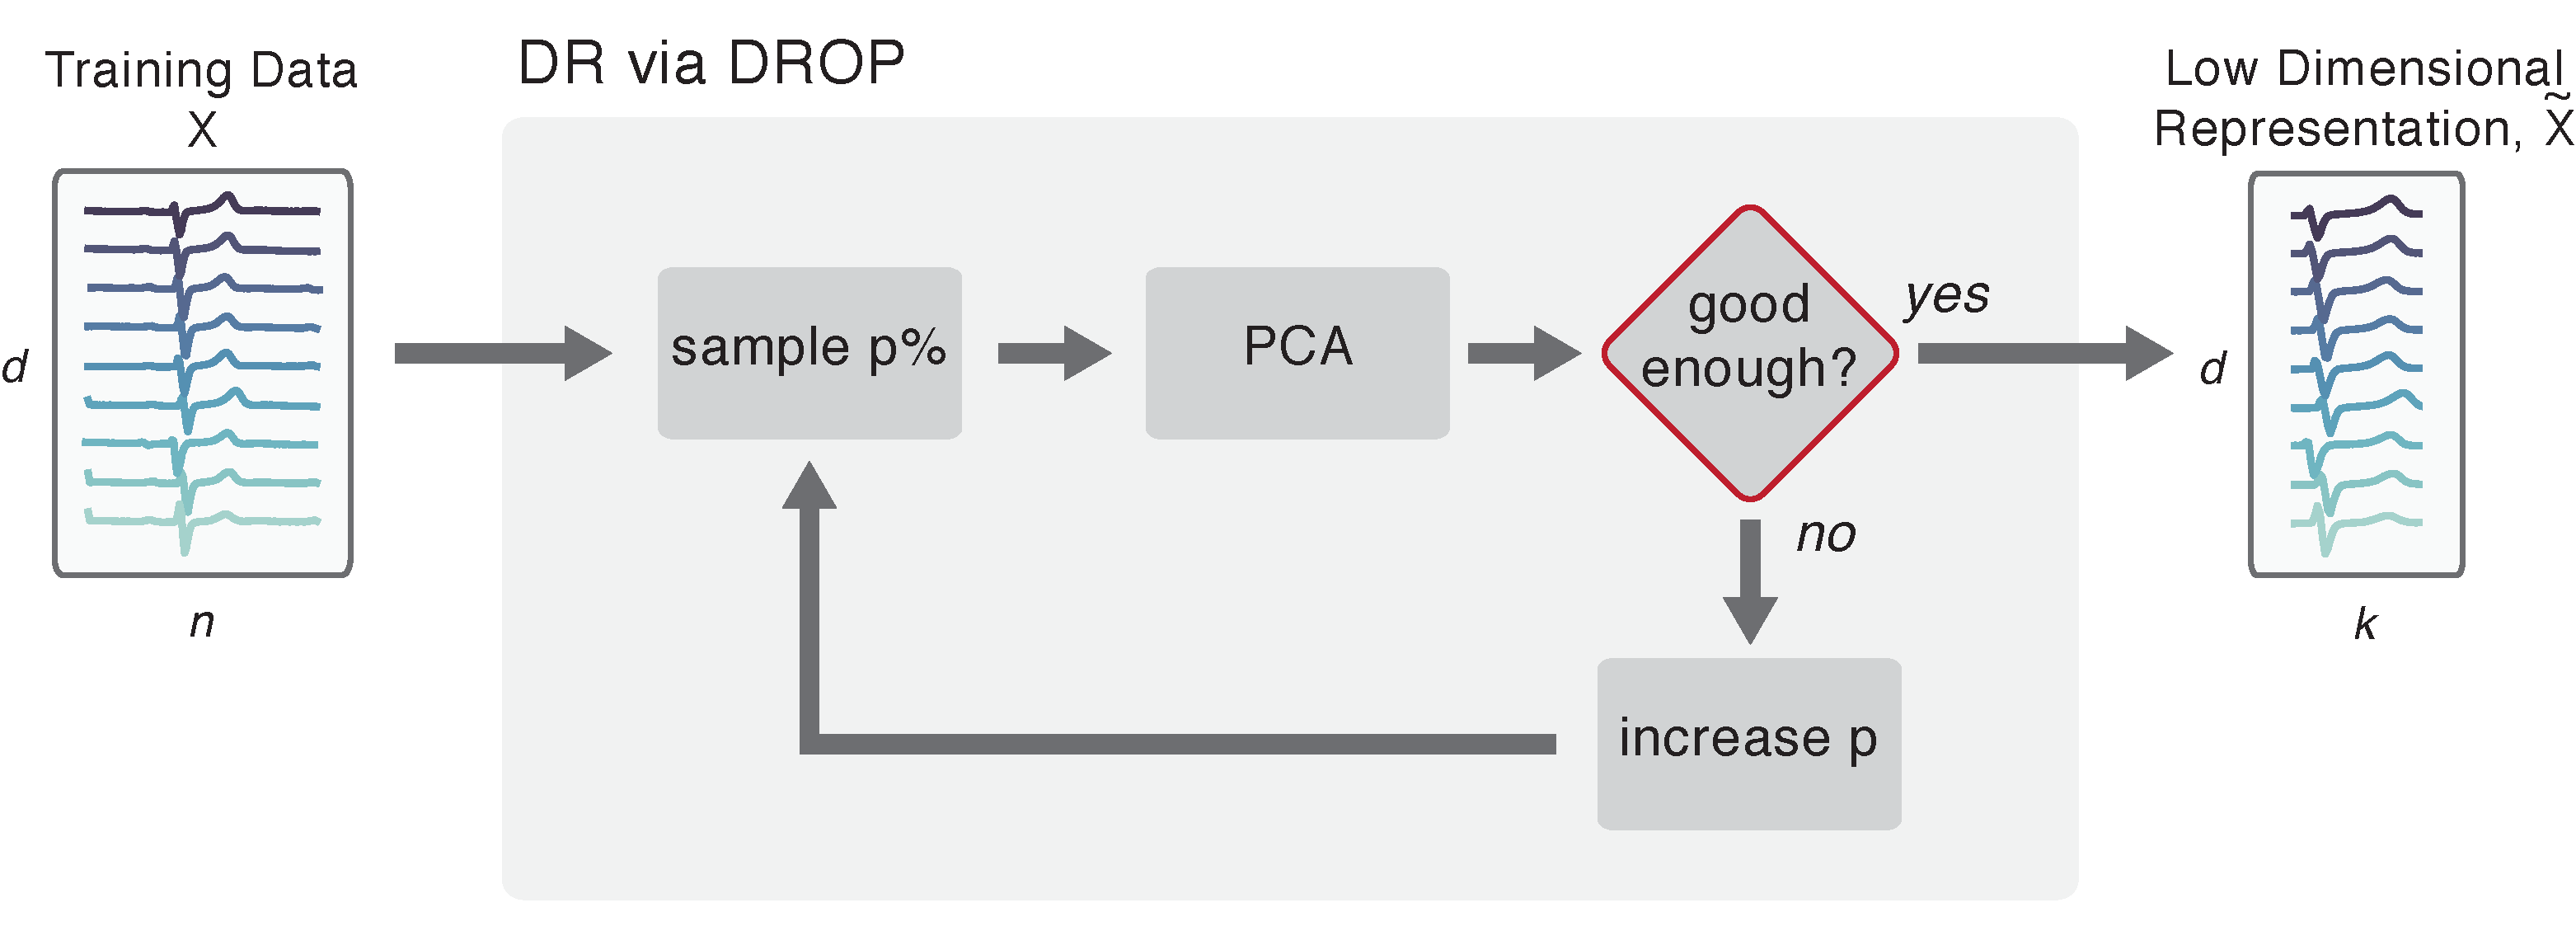
\includegraphics[width=\linewidth]{figs/basic.pdf}
\caption[]{DROP is a workload-aware PCA-based DR operator compatible with standard ML pipelines. DROP solves the challenge of when to stop sampling (``good enough?") when using sample-based stochastic PCA.}
\label{fig:basic}
\end{figure}

\begin{figure}
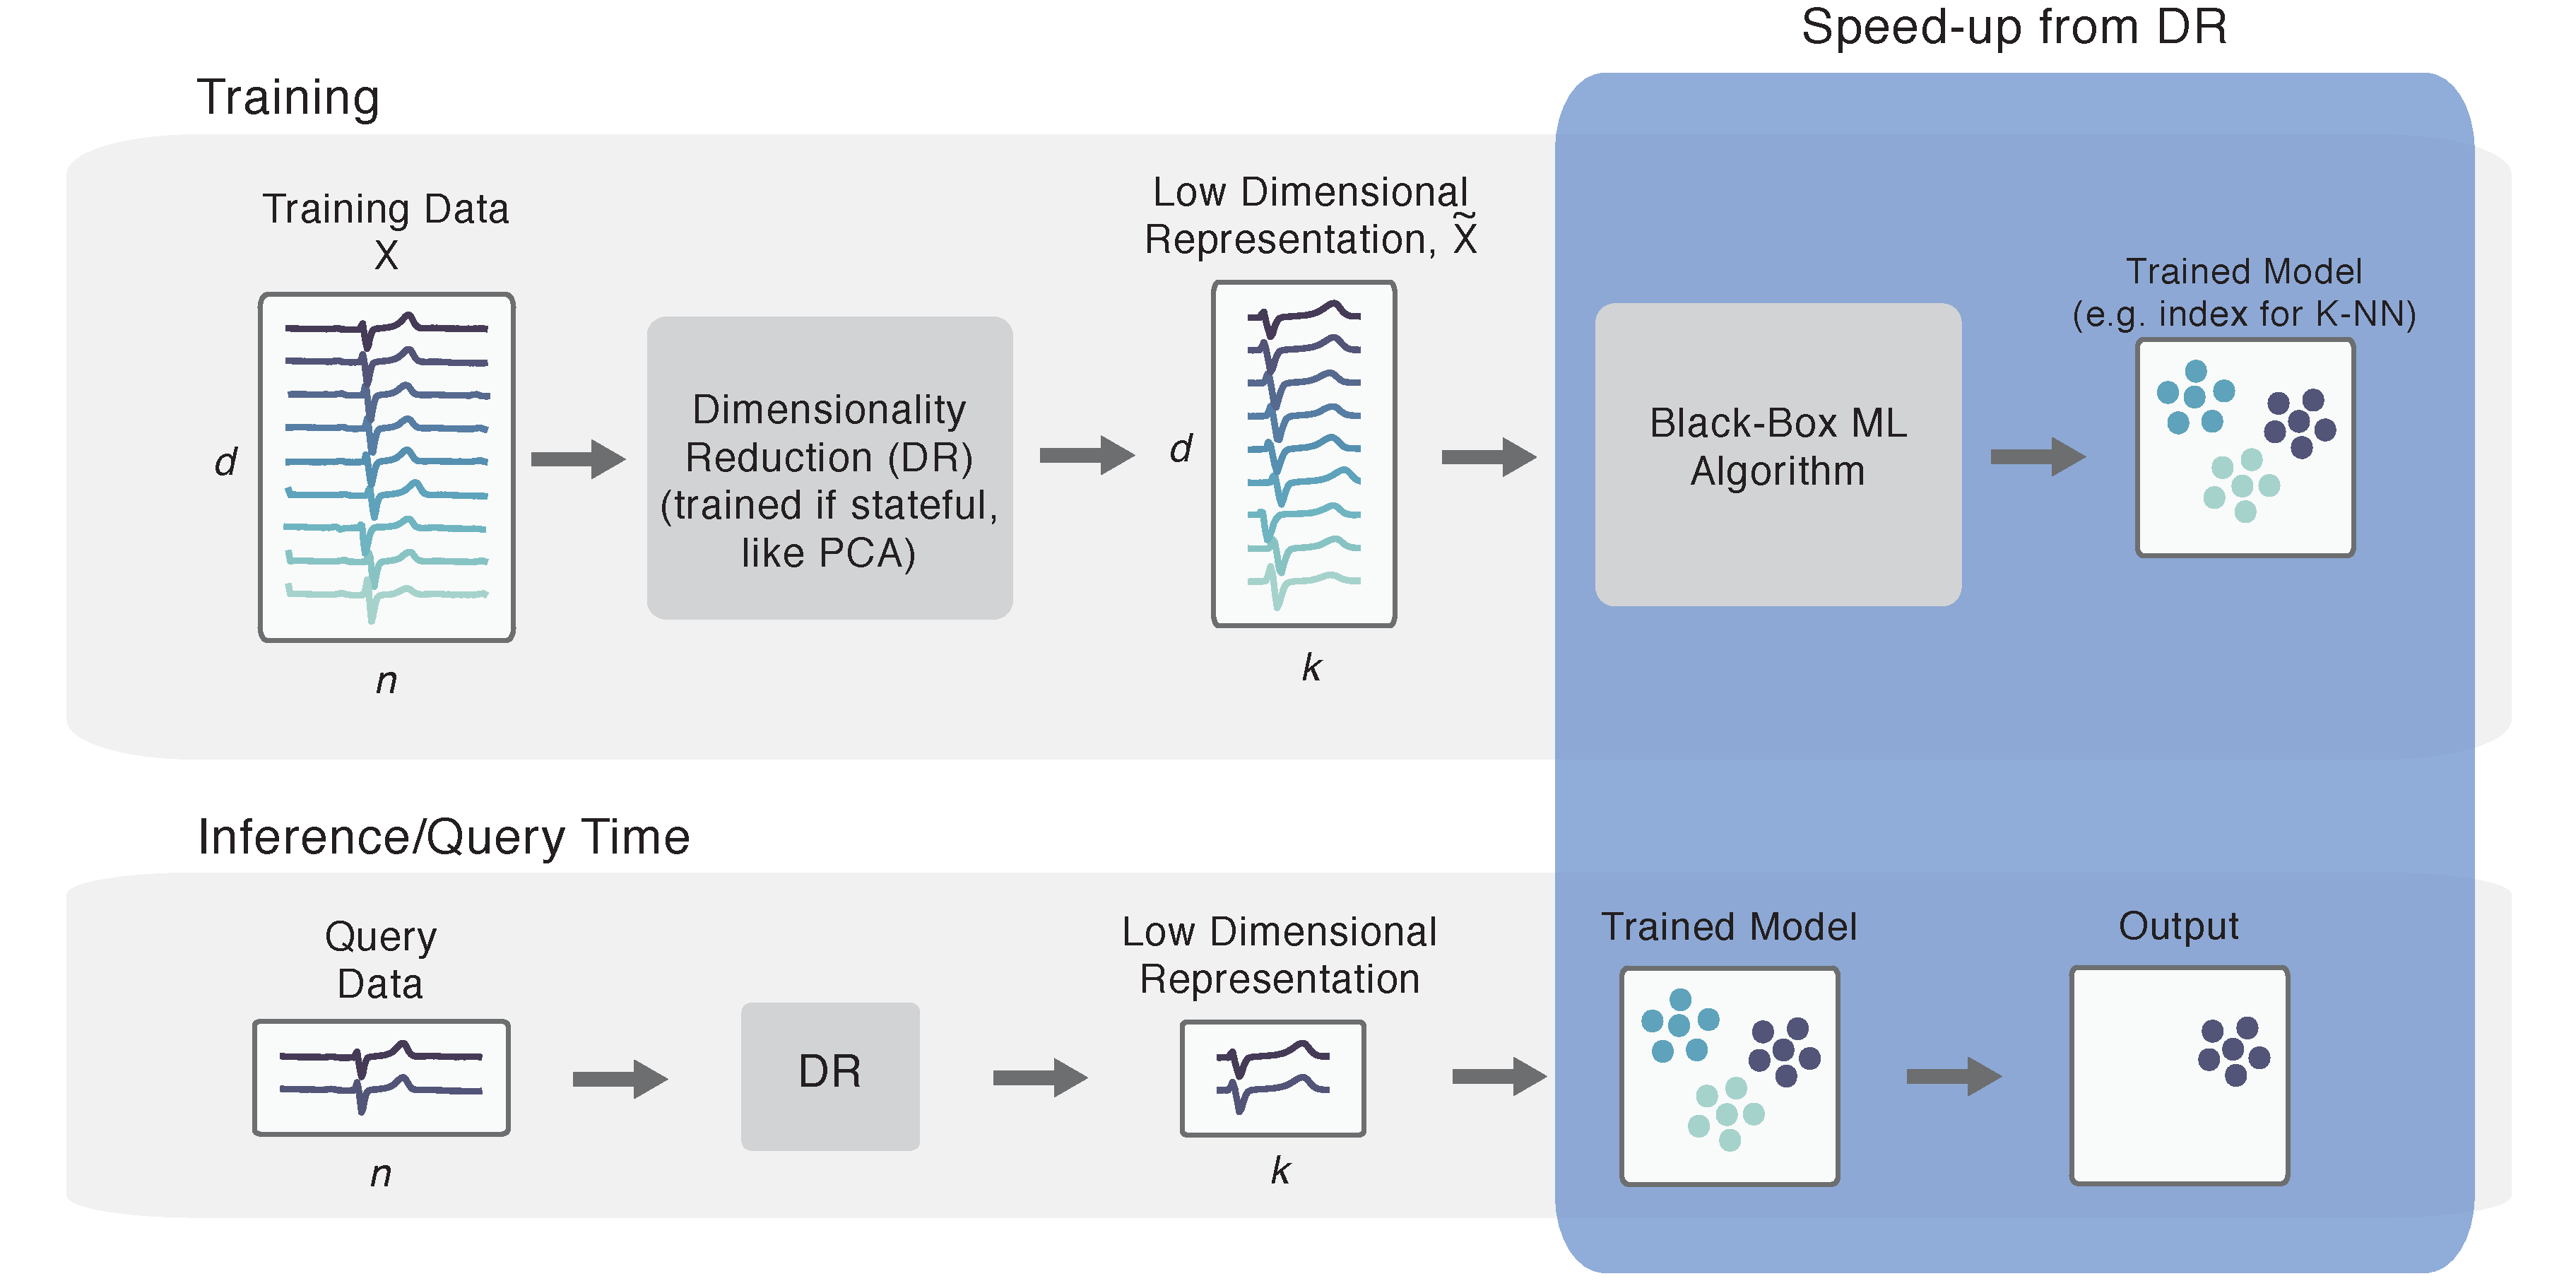
\includegraphics[width=\linewidth]{figs/pipeline.pdf}
\caption[]{Sample machine learning pipeline with dimensionality reduction. Spending time on DR provides downstream runtime speed-ups.}
\label{fig:pipeline}
\end{figure}
\end{comment}
To resolve this data- and workload-dependent trade-off, we develop DROP, a system that dynamically identifies the amount of sampling required for stochastic PCA by using downstream task information.
DROP takes as input a high-dimensional dataset,
%\footnote{Our focus \red{is on time series similarity search,} given the amount of study in the database community~\cite{keogh-study} and resurging interest in time series analytics systems~\cite{macrobase,macrobase-cidr,trill-signal}. 
%We provide preliminary generalizability analyses in \S\ref{sec:experiments}.}  
a workload-dependent constraint on approximation accuracy (e.g., pairwise Euclidean distance to 5\% for similarity search, see \S~\ref{sec:RQW}), and an optional runtime model expressing downstream computational cost as a function of dimensionality (e.g., for k-Nearest Neighbors [k-NN], runtime is linear in dimensionality). 
DROP returns a low-dimensional transformation for the input using as few samples as needed to minimize the projected overall workload runtime while preserving the input constraint. 


DROP addresses the question of how much to sample the input dataset via data-dependent progressive sampling and online progress estimation at runtime.  
DROP performs PCA on a small sample to obtain a candidate transformation, then increases the number of samples until termination. 
To identify the termination point that minimizes runtime, DROP must overcome three challenges:

First, given the results of PCA on a data sample, DROP must \emph{evaluate the quality} of the current candidate transformation.
Popular analytics and data mining tasks often require approximate preservation of metrics such as average pairwise distances between data points~\cite{time-series-dm,dm-book}, which are costly to compute.
Thus, DROP adapts confidence intervals for fast estimation of the input metric to preserve.


Second, DROP must \emph{estimate the marginal benefit of sampling additional datapoints}.
When running PCA on a series of larger samples, later samples will increase DR runtime, but may return lower $k$ (lower downstream runtime)---DROP must estimate how these values will change in future iterations to navigate this trade-off between end-to-end runtime and dimensionality.
DROP uses the results obtained from previous iterations to fit predictive models for dimensionality and runtime of the next iteration.

Finally, given the predicted marginal benefit, DROP must \emph{optimize end-to-end runtime}.
While an application-agnostic approach would iterate until successive iterations yield little or no benefit, a user-provided runtime model may reveal that trading a higher $k$ for a lower DR runtime may decrease overall runtime.
DROP evaluates the runtime model at each iteration
to minimize the expected workload runtime.


\begin{comment}

PCA is guaranteed to find the optimal linear transformation with respect to $\mathcal{L}_2$ reconstruction error, popular analytics and data mining tasks (e.g., k-NN~\cite{time-series-dm}, k-means~\cite{dm-book},  kernel density estimation~\cite{wand}) instead require approximate preservation of metrics such as average pairwise distances between data points.
To overcome this challenge, DROP adapts confidence intervals (either via closed-form or, if unavailable, via bootstrapping) for fast estimation of the input metric to preserve.


Since PCA is guaranteed to find the optimal linear transformation with respect to $\mathcal{L}_2$ reconstruction error, we could consider estimating the transformation quality using this quantity.
However, many popular analytics and data mining tasks (e.g., k-NN~\cite{time-series-dm}, k-Means~\cite{dm-book},  Kernel Density Estimation~\cite{wand}) do not use reconstruction error, and instead require approximate preservation of metrics such as average pairwise distances between data points.
A transformation that minimizes reconstruction error is not guaranteed to preserve the pairwise distance by the same amount.
Moreover, na\"ively computing pairwise distances as required for k-NN is prohibitively expensive, with quadratic runtime.
To overcome this challenge, the system adapts an approach pioneered for deterministic queries in the context of online aggregation: treat quality metrics as aggregation functions and use confidence intervals (either via closed-form or, if unavailable, via bootstrapping) for fast estimation.
This approach allows DROP to accurately estimate representation quality while avoiding the overhead of exact computation.

Second, DROP must \emph{estimate the marginal benefit of continuing to sample} for another iteration.
When running PCA on a series of progressively larger samples, later samples will incur higher computational cost but may in turn return lower-dimensional transformations. 
To navigate this trade-off between end-to-end runtime and transformation quality, the system performs online progress estimation, using the results obtained from previous iterations to build a predictive performance model for future iterations.
%This allows DROP to quantify the expected benefit of continued sampling.

Finally, given the current quality and expected marginal benefit of the next iteration, DROP must \emph{optimize end-to-end runtime} to determine whether to terminate.  
The system must evaluate if the expected marginal benefit to dimensionality arising from continuing to iterate would reduce total runtime.
While an application-agnostic approach would iterate until successive iterations yield no benefit to quality, many analytics operators such as k-Nearest Neighbors are tolerant of error~\cite{gemini}, so it is frequently advantageous to trade a slightly higher-dimensional basis for faster pre-processing (DR).
To address this challenge, the system performs workload-specific optimization to minimize the expected runtime of the complete end-to-end analytics pipeline.
\end{comment}

\begin{comment}
A simple, application-agnostic approach to addressing this problem would iterate until until successive iterations yield no benefit to quality, thus converging to the lowest-dimensional metric-preserving transformation.
However, as we have hinted, many time-series analytics operators such as k-Nearest Neighbors are tolerant of approximation error~\cite{gemini}, and it is frequently advantageous to trade a slightly higher-dimensional basis for faster pre-processing. In these settings, running to convergence is often wasteful.
To address this challenge, DROP performs a workload-specific optimization, utilizing a provided (or profiled) application-specific runtime model and performs online optimization  to minimize the expected runtime of the complete end-to-end analytics pipeline.
\end{comment} 

DROP is a system that combines recent theoretical advances in DR and classic techniques from approximate query processing for end-to-end workflow optimization.
In this work, we make the following contributions:
\begin{itemize}

\item We show the data sample required to perform accuracy-achieving PCA is often small (as little as $1\%$), and sampling can enable up to \red{$91\times$} speedup over baseline PCA. 
%We show that as little as $2\%$ of time series data suffices to preserve pairwise distances within $2\%$, providing a $55.6\times$ reduction in dimension.
  %this came from the oracle numbers--used 0.002 and then looked at table
  
\item We propose DROP, an online optimizer for DR that uses information about downstream analytics tasks to perform efficient stochastic PCA.
%. DROP uses information about downstream analytics tasks to utilize as few samples as required to minimize the overall workload runtime, while satisfying constraints on the reduction quality.

\item We present techniques based on progressive sampling, approximate query processing, online progress estimation, and cost based optimization to enable up to \red{$5\times$} faster end-to-end execution over PCA via SVD.% and up to $3\times$ faster end-to-end execution than alternative techniques on real analytics pipelines.
\end{itemize}



